%!TEX root = ../Master.tex
\section{Results}\label{sec:results}
%\subsection{Data rate}
We see that the packet loss at a specific TxR does not depend on distance between the sender and receiver given the bounderies of the scenario\cite{rangetest}. Table \ref{tbl:measuredThroughput} shows the UDP SDU throughtput, as measured in \cite{WorksheetThroughput}.
The measured TxR of Table \ref{tbl:measuredThroughput} are not only subject to protocol design limitations, but might also be affected by other traffic on the link e.g. beacons from the access point and interference from other 802.11 devices all of which decreases the application throughput.
\begin{table}[ht]
\centering
\begin{tabular}{c|c}
TxR & \begin{tabular}[c]{@{}l@{}}UDP  SDU throughput\end{tabular} \\ \hline
12 Mb/s   & 10.296 Mb/s                                                                                    \\
18 Mb/s   & 14.958 Mb/s                                                                                    \\
24 Mb/s   & 19.305 Mb/s                                                                                    \\
36 Mb/s   & 27.174 Mb/s
\end{tabular}
\caption{TxR specified in 802.11g and the equivalent throughput measured at the application layer}
\label{tbl:measuredThroughput}
\end{table}

As expected the application data rate is lower than the MxR and it is something that should be considered not only when adjusting the reliability parameters but also when examining the system delay.

%\subsection{Video encoding}
Segments of three video traces captured by the drone at 5, 10, 20 Mb/s can be seen in Figure \ref{fig:vtrace}. Each dot indicate the arrival of a new frame and the height indicate the bitrate needed to service the frame before a new frame arrives. As seen in the Figure \ref{fig:vtrace}, the VBR encoding mechanism allocates much of the available bandwidth for the I-frame which is depicted by the spike. The I-frame is a full frame and not incremental differences as the next frames and it has a period of 1 second at 30 fps.

\begin{figure}[ht]
	\centering
	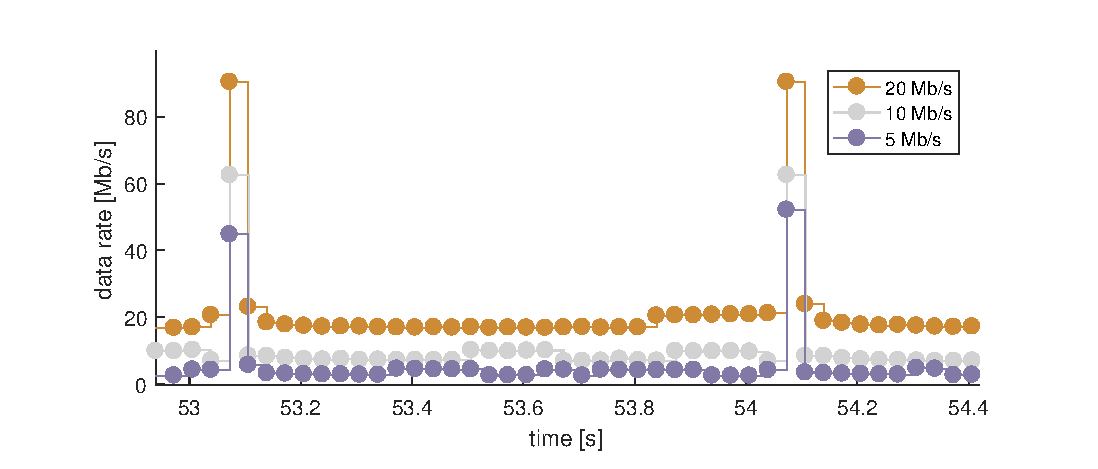
\includegraphics[width=\linewidth]{images/vids.eps}
	\caption{Traces of different three H.264 encoded VBR videos at different target bitrates}
	\label{fig:vtrace}
\end{figure}
\begin{figure}[ht]
	\centering
	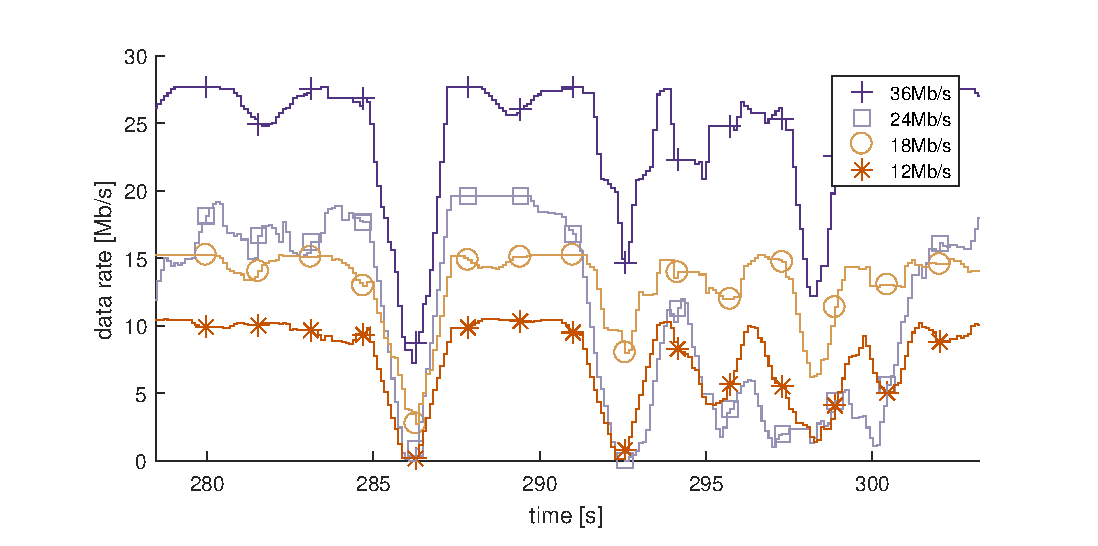
\includegraphics[width=\linewidth]{images/traceAvg10.eps}
	\caption{Available throughput obtained in a trace of different TxR}
	\label{fig:trace}
\end{figure}

The next result, seen in Figure \ref{fig:trace}, are traces showing the estimated behaviour of the different TxR. It shows that the rates are correlated, which means that the errors we observe are not rate specific. The reasons for the decreasing throughput, could be caused by a combination of the following reasons: (i) the sender gets out of range of the receiver, (ii) background noise, (iii) nearby transmission equipment is causing noise or (iv) the drones movement, e.g. acceleration distorts the transmitted signal. Of the mentioned reasons we suspect a combination of reason (i), (ii) and (iv) to be causing the majority of the throughput decrease we see in the traces in Figure \ref{fig:trace}. Furthermore, it is seen that the highest TxR still offers the highest throughput.
